\documentclass[journal=jacsat,manuscript=article]{achemso}\usepackage[]{graphicx}\usepackage[]{color}
% maxwidth is the original width if it is less than linewidth
% otherwise use linewidth (to make sure the graphics do not exceed the margin)
\makeatletter
\def\maxwidth{ %
  \ifdim\Gin@nat@width>\linewidth
    \linewidth
  \else
    \Gin@nat@width
  \fi
}
\makeatother

\definecolor{fgcolor}{rgb}{0.345, 0.345, 0.345}
\newcommand{\hlnum}[1]{\textcolor[rgb]{0.686,0.059,0.569}{#1}}%
\newcommand{\hlstr}[1]{\textcolor[rgb]{0.192,0.494,0.8}{#1}}%
\newcommand{\hlcom}[1]{\textcolor[rgb]{0.678,0.584,0.686}{\textit{#1}}}%
\newcommand{\hlopt}[1]{\textcolor[rgb]{0,0,0}{#1}}%
\newcommand{\hlstd}[1]{\textcolor[rgb]{0.345,0.345,0.345}{#1}}%
\newcommand{\hlkwa}[1]{\textcolor[rgb]{0.161,0.373,0.58}{\textbf{#1}}}%
\newcommand{\hlkwb}[1]{\textcolor[rgb]{0.69,0.353,0.396}{#1}}%
\newcommand{\hlkwc}[1]{\textcolor[rgb]{0.333,0.667,0.333}{#1}}%
\newcommand{\hlkwd}[1]{\textcolor[rgb]{0.737,0.353,0.396}{\textbf{#1}}}%
\let\hlipl\hlkwb

\usepackage{framed}
\makeatletter
\newenvironment{kframe}{%
 \def\at@end@of@kframe{}%
 \ifinner\ifhmode%
  \def\at@end@of@kframe{\end{minipage}}%
  \begin{minipage}{\columnwidth}%
 \fi\fi%
 \def\FrameCommand##1{\hskip\@totalleftmargin \hskip-\fboxsep
 \colorbox{shadecolor}{##1}\hskip-\fboxsep
     % There is no \\@totalrightmargin, so:
     \hskip-\linewidth \hskip-\@totalleftmargin \hskip\columnwidth}%
 \MakeFramed {\advance\hsize-\width
   \@totalleftmargin\z@ \linewidth\hsize
   \@setminipage}}%
 {\par\unskip\endMakeFramed%
 \at@end@of@kframe}
\makeatother

\definecolor{shadecolor}{rgb}{.97, .97, .97}
\definecolor{messagecolor}{rgb}{0, 0, 0}
\definecolor{warningcolor}{rgb}{1, 0, 1}
\definecolor{errorcolor}{rgb}{1, 0, 0}
\newenvironment{knitrout}{}{} % an empty environment to be redefined in TeX

\usepackage{alltt}\usepackage[]{graphicx}\usepackage[]{color}
%% maxwidth is the original width if it is less than linewidth
%% otherwise use linewidth (to make sure the graphics do not exceed the margin)
\makeatletter
\def\maxwidth{ %
  \ifdim\Gin@nat@width>\linewidth
    \linewidth
  \else
    \Gin@nat@width
  \fi
}
\makeatother


\usepackage{subfig}
\usepackage{graphicx}
\usepackage{alltt}

\usepackage{chemformula} % Formula subscripts using \ch{}
\usepackage[T1]{fontenc} % Use modern font encodings

%%%%%%%%%%%%%%%%%%%%%%%%%%%%%%%%%%%%%%%%%%%%%%%%%%%%%%%%%%%%%%%%%%%%%
%% If issues arise when submitting your manuscript, you may want to
%% un-comment the next line.  This provides information on the
%% version of every file you have used.
%%%%%%%%%%%%%%%%%%%%%%%%%%%%%%%%%%%%%%%%%%%%%%%%%%%%%%%%%%%%%%%%%%%%%
%%\listfiles

\newcommand*\mycommand[1]{\texttt{\emph{#1}}}

\author{Laurent Gatto}
\email{laurent.gatto@uclouvain.be}
\affiliation[UCLouvain]{Computational Biology Unit, de Duve Institute, Universit\'e catholique de Louvain, Brussels, Belgium}
\author{Sebastian Gibb}
\affiliation[University of Greifswald]{Department of Anaesthesiology and Intensive Care of the University Medicine Greifswald, Germany}
\author{Johannes Rainer}
\affiliation[Eurac Research]{Institute for Biomedicine, Eurac Research, Affiliated Institute of the University of L\"ubeck, Bolzano, Italy}


\title[MSnbase version 2]
  {\texttt{MSnbase}, efficient and elegant R-based processing and
    visualisation of raw mass spectrometry data}

\abbreviations{}
\keywords{Bioconductor, mass spectrometry, software, metabolomics, proteomics, visualisation, reproducible research} %% up to 10 keywords
\IfFileExists{upquote.sty}{\usepackage{upquote}}{}
\IfFileExists{upquote.sty}{\usepackage{upquote}}{}
\begin{document}

%% \begin{tocentry}
%% See achemso-demo.tex
%% \end{tocentry}

\begin{abstract} %% 200 words max
  We present version 2 of the \texttt{MSnbase} R/Bioconductor
  package. \texttt{MSnbase} provides infrastructure for the
  manipulation, processing and visualisation of mass spectrometry
  data. We focus on the new \textit{on-disk} infrastructure, that
  allows the handling of large raw mass spectrometry experiment on
  commodity hardware and illustrate how the package is used for
  elegant data processing, method development and visualisation.
\end{abstract}



\section{Introduction}

Mass spectrometry is a powerful technology to assay chemical and
biological samples. It is used in routine with well characterised
protocol, as well a development platform, to improve on existing
methods and devise new ones. The complexity and diversity of mass
spectrometry yield data that is itself complex and often times of
considerable size, that require non trivial processing before
producing interpretable results. This is particularly relevant, and
can constitute a significant challenge for method development: in
addition to the development of sample processing and mass spectrometry
methods, there is a need to process, analyse, interpret and assess
these new data to demonstrate the improvement in the technical,
analytical and computational workflows.

Practitioners have a diverse catalogue of software tools to explore,
process and interpret mass spectrometry data at their disposal. These
range from low level software libraries that are aimed at programmers
to enable development of new applications, to more user-oriented
applications with graphical user interfaces which provide a more
limited set of functionalities to address a defined scope. Examples of
software libraries include Java-based jmzML~\cite{Cote:2010} or
C/C++-based ProteoWizard~\cite{Chambers:2012}. ProteomeDiscoverer
(Thermo Scientific), MaxQuant~\cite{Cox:2008} and
PeptideShaker~\cite{Vaudel:2015} are among the most widely used
user-centric applications.

In this software note, we present version 2 of the \texttt{MSnbase}
\cite{Gatto:2012} software, available from the
Bioconductor~\cite{Huber:2015} project. \texttt{MSnbase}, like other
software such as Python-based {pyOpenMS}~\cite{Rost:2014},
spectrum\_utils~\cite{Bittremieux:2020} or
Pyteomics~\cite{Goloborodko:2013}, offers a platform that lies between
low level libraries and end-user software. \texttt{MSnbase} provides a
flexible R~\cite{R} command line environment for metabolomics and
proteomics mass spectrometry-based applications. It allows a detailed
step-by-step processing, analysis and exploration of the data and
development of novel computational mass spectrometry
methods~\cite{Stanstrup:2019}.

\section{Software functionality}

In \texttt{MSnbase}, mass spectrometry experiments are handled as
\texttt{MSnExp} objects. While the implementation is more complex, it
is useful to schematise a raw data experiment as being composed of raw
data, i.e. a collection of individual spectra, as well as
spectra-level metadata. Each spectrum is composed of m/z values and
associated intensities. The metadata are represented by a table with
variables along the columns and each row associated to a
spectrum. Among the metadata available for each spectrum, there are MS
level, acquisition number, retention time, precursor m/z and intensity
(for MS level 2 and above), and many more. \texttt{MSnbase} provides a
rich interface to manipulate such objects. The code chunk below
illustrates such an object as displayed in the R console and an
enumeration of the metadata fields.

\begin{knitrout}
\definecolor{shadecolor}{rgb}{0.969, 0.969, 0.969}\color{fgcolor}\begin{kframe}
\begin{alltt}
> \hlkwd{show}(ms)
MSn experiment \hlkwd{data} (\hlstr{"OnDiskMSnExp"})
Object size in memory: 0.54 Mb
- - - Spectra data - - -
 MS \hlkwd{level}(s): 1 2 3 
 Number of spectra: 994 
 MSn retention times: 45:27 - 47:6 minutes
- - - Processing information - - -
Data loaded [Sun Apr 26 15:40:58 2020] 
 MSnbase version: 2.13.6 
- - - Meta data  - - -
phenoData
  rowNames: MS3TMT11.mzML
  varLabels: sampleNames
  varMetadata: labelDescription
Loaded from:
  MS3TMT11.mzML 
protocolData: none
featureData
  featureNames: F1.S001 F1.S002 ... \hlkwd{F1.S994} (994 total)
  fvarLabels: fileIdx spIdx ... \hlkwd{spectrum} (35 total)
  fvarMetadata: labelDescription
experimentData: use \hlstr{'\hlkwd{experimentData}(object)'}
> \hlkwd{fvarLabels}(ms)
 [1] \hlstr{"fileIdx"}                    \hlstr{"spIdx"}
 [3] \hlstr{"smoothed"}                   \hlstr{"seqNum"}
 [5] \hlstr{"acquisitionNum"}             \hlstr{"msLevel"}
 [7] \hlstr{"polarity"}                   \hlstr{"originalPeaksCount"}
 [9] \hlstr{"totIonCurrent"}              \hlstr{"retentionTime"}
[11] \hlstr{"basePeakMZ"}                 \hlstr{"basePeakIntensity"}
[13] \hlstr{"collisionEnergy"}            \hlstr{"ionisationEnergy"}
[15] \hlstr{"lowMZ"}                      \hlstr{"highMZ"}
[17] \hlstr{"precursorScanNum"}           \hlstr{"precursorMZ"}
[19] \hlstr{"precursorCharge"}            \hlstr{"precursorIntensity"}
[21] \hlstr{"mergedScan"}                 \hlstr{"mergedResultScanNum"}
[23] \hlstr{"mergedResultStartScanNum"}   \hlstr{"mergedResultEndScanNum"}
[25] \hlstr{"injectionTime"}              \hlstr{"filterString"}
[27] \hlstr{"spectrumId"}                 \hlstr{"centroided"}
[29] \hlstr{"ionMobilityDriftTime"}       \hlstr{"isolationWindowTargetMZ"}
[31] \hlstr{"isolationWindowLowerOffset"} \hlstr{"isolationWindowUpperOffset"}
[33] \hlstr{"scanWindowLowerLimit"}       \hlstr{"scanWindowUpperLimit"}
[35] \hlstr{"spectrum"}
\end{alltt}
\end{kframe}
\end{knitrout}

In the following sections, we describe \texttt{MSnbase}'s ability to efficiently
manage very large mass spectrometry data and experiments and how it can be used
for data processing and visualisation. We will also illustrate how it makes use
of the forward-pipe operator (\texttt{\%>\%}) defined in the \texttt{magrittr}
package. This operator has proved useful to develop non-trivial analyses by
combining individual functions into easily readable pipelines.

\subsection{On-disk backend}

The main feature in version 2 of the \texttt{MSnbase} package was the
addition of different backends for raw data storage, namely
\textit{in-memory} and \textit{on-disk}. The following code chunk
demonstrates how to create two \texttt{MSnExp} objects storing data
either in-memory or on-disk. Both modes rely on the
\texttt{mzR}~\cite{Chambers:2012} package to access the data in the
raw data files.

\begin{knitrout}
\definecolor{shadecolor}{rgb}{0.969, 0.969, 0.969}\color{fgcolor}\begin{kframe}
\begin{alltt}
\hlkwd{library}\hlstd{(}\hlstr{"MSnbase"}\hlstd{)}
\hlstd{raw_mem} \hlkwb{<-} \hlkwd{readMSData}\hlstd{(}\hlstr{"file.mzML"}\hlstd{,} \hlkwc{mode} \hlstd{=} \hlstr{"inMemory"}\hlstd{)}
\hlstd{raw_dsk} \hlkwb{<-} \hlkwd{readMSData}\hlstd{(}\hlstr{"file.mzML"}\hlstd{,} \hlkwc{mode} \hlstd{=} \hlstr{"onDisk"}\hlstd{)}
\end{alltt}
\end{kframe}
\end{knitrout}







\begin{figure}[p]
  \centering
\begin{knitrout}
\definecolor{shadecolor}{rgb}{0.969, 0.969, 0.969}\color{fgcolor}
\includegraphics[width=\maxwidth]{figure/plot_bench-1} 

\end{knitrout}
\caption{(a) Reading time (in seconds) and (b) data size in memory (in
  MB) to read/store 1, 5 and 10 files containing 1431 MS1 (on-disk
  only) and 6103 MS2 (on-disk and in-memory) spectra. (c) Filtering
  benchmark assessed over 10 interactions on in-memory and on-disk data
  containing 6103 MS2 spectra.  (d) Access time to spectra for the
  in-memory (left) and on-disk (right) backends for 1, 10, 100 1000,
  5000 and all 6103 spectra. On-disk backend: blue. In-memory backend:
  red. }
\label{fig:bench}
\end{figure}


The former is the legacy storage mode, implemented in the first
version of the package, that loads all the raw data and the metadata
into memory. This solution doesn't scale for modern large dataset, and
was complemented by the on-disk backend. The on-disk backend loads the
metadata into memory and accesses the spectra data (i.e. m/z and
intensity values) in the original files only when needed. There are
two direct benefits using the on-disk backend, namely faster reading
and reduced memory footprint. Figure \ref{fig:bench} shows 5-fold
faster reading times (a) and over a 10-fold reduction in memory usage
(b).

The on-disk backend also offers efficient data manipulation by way of
\textit{lazy processing}. Operations on the raw data are stored in a
processing queue and only effectively applied when the user accesses m/z or
intensity values. As an example, the following short analysis
pipeline, that can equally be applied to in-memory or on-disk data,
retains MS2 spectra acquired between 1000 and 3000 seconds, extracts
the m/z range corresponding to the TMT 6-plex range and focuses on the
MS2 spectra with a precursor intensity greater than $11 \times 10^6$
(the median precursor intensity). 

\begin{knitrout}
\definecolor{shadecolor}{rgb}{0.969, 0.969, 0.969}\color{fgcolor}\begin{kframe}
\begin{alltt}
\hlstd{ms} \hlkwb{<-} \hlstd{ms} \hlopt
    \hlkwd{filterRt}\hlstd{(}\hlkwd{c}\hlstd{(}\hlnum{1000}\hlstd{,} \hlnum{3000}\hlstd{))} \hlopt
    \hlkwd{filterMz}\hlstd{(}\hlnum{120}\hlstd{,} \hlnum{135}\hlstd{)}
\hlstd{ms[}\hlkwd{precursorIntensity}\hlstd{(ms)} \hlopt{>} \hlnum{11e6}\hlstd{, ]}
\end{alltt}
\end{kframe}
\end{knitrout}

As shown on Figure~\ref{fig:bench} (c), this lazy mechanism is
significantly faster than its application on in-memory data. The
advantageous reading and execution times and memory footprint of the
on-disk backend are possible by retrieving only spectra data from the selected
subset hence avoiding access to the full raw
data. Once access to the spectra m/z and intensity values become
mandatory (for example for plotting), then the in-memory backend
becomes more efficient, as illustrated on Figure~\ref{fig:bench}
(d). This gain is maximal when the whole dataset is accessed
(i.e. all spectra are already in memory) and negligible when only subsets of the
data are requested.


\subsection{Prototyping}

The \texttt{MSnExp} data structure and its interface constitute a
efficient prototyping environment for computational method
development. We illustrate this by demonstrating how to implement the
BoxCar\cite{Meier:2018} acquisition method. In a nutshell, BoxCar
acquisition aims at improving the detection of intact precursor ions
by distributing the charge capacity over multiple narrow m/z segments
and thus limiting the proportion of highly abundant precursors in each
segment. A full scan is reconstructed by combining the respective
adjacent segments of the BoxCar acquisitions. The
\texttt{MSnbaseBoxCar} package\cite{MSnbaseBoxCar} is a small package
that demonstrates this. The simple method is composed of three steps
is described below and illustrated with code from
\texttt{MSnbaseBoxCar} in the following code chunk.

\begin{enumerate}

\item Identify and filter the groups of spectra that represent
  adjacent BoxCar acquisitions (Figure~\ref{fig:bc}~(b)). This can be
  done using the \textit{filterString} metadata variable that
  identifies BoxCar spectra by their adjacent m/z segments with the
  \texttt{bc\_groups()} function and filtering relevant spectra with
  the \texttt{filterBoxCar()}.
  
\item Remove any signal outside the BoxCar segments using the
  \texttt{bc\_zero\_out\_box()} function from \texttt{MSnbaseBoxCar}
  (Figures~\ref{fig:bc}~(c) and (d)).


\item Using the \texttt{combineSpectra} function from the
  \texttt{MSnbase}, combine the cleaned BoxCar spectra into a new,
  full spectrum (Figure~\ref{fig:bc}~(e)).

\end{enumerate}

\begin{knitrout}
\definecolor{shadecolor}{rgb}{0.969, 0.969, 0.969}\color{fgcolor}\begin{kframe}
\begin{alltt}
\hlstd{bc} \hlkwb{<-} \hlkwd{readMSData}\hlstd{(}\hlstr{"boxcar.mzML"}\hlstd{,} \hlkwc{mode} \hlstd{=} \hlstr{"onDisk"}\hlstd{)} \hlopt
      \hlkwd{bc_groups}\hlstd{()} \hlopt       \hlcom{## identify BoxCar groups (bc_groups)}
      \hlkwd{filterBoxCar}\hlstd{()} \hlopt    \hlcom{## keep only BoxCar spectra}
      \hlkwd{bc_zero_out_box}\hlstd{()} \hlopt \hlcom{## remove signal outside of BoxCar segments}
      \hlkwd{combineSpectra}\hlstd{(}\hlkwc{fcol} \hlstd{=} \hlstr{"bc_groups"}\hlstd{,} \hlcom{## reconstruct full spectrum}
                     \hlkwc{method} \hlstd{= boxcarCompbine)}
\end{alltt}
\end{kframe}
\end{knitrout}



\begin{figure}[p]
  \centering
\begin{knitrout}
\definecolor{shadecolor}{rgb}{0.969, 0.969, 0.969}\color{fgcolor}
\includegraphics[width=\maxwidth]{figure/plot_boxcar-1} 

\end{knitrout}
\caption{BoxCar processing with \texttt{MSnbase}. (a) Standard full
  scan with (b) three corresponding BoxCar scans showing the adjacent
  segments. Figure (c) shows the overlapping intact BoxCar segments
  and (d) the same segments after cleaning, i.e. where peaks outside
  of the segments were removed. The reconstructed full scan is shown
  on panel (e).}
\label{fig:bc}
\end{figure}

All the functions for the processing of BoxCar spectra and segments in
\texttt{MSnbaseBoxCar} were developed using existing functionality
implemented in \texttt{MSnbase}, illustrating the flexibility and
adaptability of the \texttt{MSnbase} package for computational mass
spectrometry method development.


\subsection{Visualisation}

The R environment is well known for the quality of its visualisation
capacity. This also holds true for mass
spectrometry\cite{Gatto:2015,protViz,Pviz,Bemis:2015}. Here, we
conclude the overview of version 2 of the \texttt{MSnbase} package by
highlighting the flexibility of the software to visualise and assess
the efficiency of raw data processing. Figure \ref{fig:cent} compares
the raw MS profile data for the serine and the same data after
smoothing, centroiding and m/z refinement, as illustrated in the code
chunk below. Detailed execution and description of these operations
can be found in the \emph{MSnbase: centroiding of profile-mode MS
  data} \texttt{MSnbase} vignette.

\begin{knitrout}
\definecolor{shadecolor}{rgb}{0.969, 0.969, 0.969}\color{fgcolor}\begin{kframe}
\begin{alltt}
\hlstd{serine_mz} \hlkwb{<-} \hlnum{106.049871}
\hlstd{serine_proc} \hlkwb{<-} \hlstd{ms} \hlopt
    \hlkwd{smooth}\hlstd{(}\hlkwc{method} \hlstd{=} \hlstr{"SavitzkyGolay"}\hlstd{,} \hlkwc{halfWindowSize} \hlstd{=} \hlnum{4L}\hlstd{)} \hlopt
    \hlkwd{pickPeaks}\hlstd{(}\hlkwc{refineMz} \hlstd{=} \hlstr{"descendPeak"}\hlstd{)} \hlopt
    \hlkwd{filterRt}\hlstd{(}\hlkwd{c}\hlstd{(serine_mz} \hlopt{-} \hlnum{0.01}\hlstd{, serine_mz} \hlopt{+} \hlnum{0.01}\hlstd{))} \hlopt
    \hlkwd{filterMz}\hlstd{(}\hlkwd{c}\hlstd{(}\hlnum{175}\hlstd{,} \hlnum{187}\hlstd{))}
\end{alltt}
\end{kframe}
\end{knitrout}

\begin{figure}
  \centering
  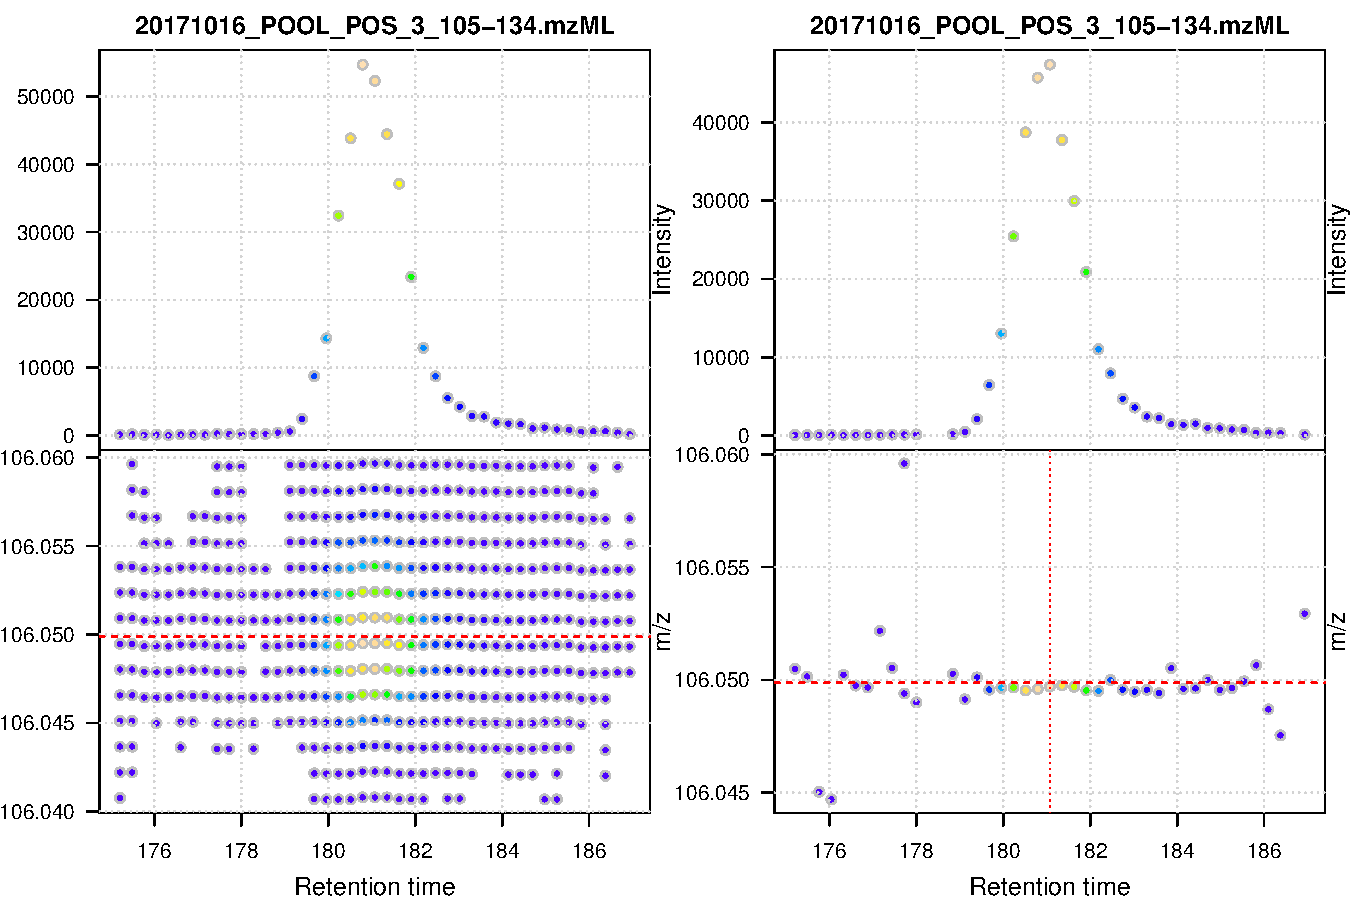
\includegraphics[width=\linewidth]{./figure/centroiding.pdf}
  \caption{Visualisation of data smoothing and m/z refinement using
    \texttt{MSnbase}. (a) Raw MS profile data for serine. Upper panel
    shows the base peak chromatogram (BPC), lower panel the individual
    signals in the retention time -- m/z space. The horizontal dashed
    red line indicates the theoretical m/z of the [M+H]+ adduct of
    serine. (b) Smoothed and centroided data for serine with m/z
    refinement. The horizontal red dashed line indicates the
    theoretical m/z for the [M+H]+ ion and the vertical red dotted
    line the position of the maximum signal. }
  \label{fig:cent}
\end{figure}


\section{Discussion}

We have presented here some some important functionality of
\texttt{MSnbase} version 2. The new on-disk infrastructure enables
large scale data analyses~\cite{Nothias:2020}, either using
\texttt{MSnbase} directly or through packages that rely on it, such as
\texttt{xcms}. We have also illustrated how \texttt{MSnbase} can be
used for standard data analysis and visualisation, and how it can be
used for method development and prototyping.

The first public commit to the \texttt{MSnbase} GitHub repository was
in October 2010. Since then, the package benefited from 12
contributors\cite{contribs} that added various features, some
particularly significant ones such as the on-disk backend described
herein. According to \texttt{MSnbase}'s Bioconductor page, there are
36 Bioconductor packages that depend, import or suggest it. Among
these are \texttt{pRoloc}~\cite{Gatto:2014a} to analyse mass
spectrometry-based spatial proteomics data,
\texttt{msmsTests}~\cite{msmsTests}, \texttt{DEP}~\cite{Zhang:2018},
\texttt{DAPAR} and \texttt{ProStaR}~\cite{Wieczorek:2017} for the
statistical analysis for quantitative proteomics data,
\texttt{RMassBank}~\cite{Stravs:2013} to process metabolomics tandem
MS files and build MassBank records,
\texttt{MSstatsQC}~\cite{Dogu:2017} for longitudinal system
suitability monitoring and quality control of targeted proteomic
experiments and the widely used \texttt{xcms}~\cite{Smith:2006} package
for the processing and analysis of metabolomics data. \texttt{MSnbase}
is also used in non-R/Bioconductor software, such as for example
IsoProt~\cite{Griss:2019}, that provides a reproducible workflow for
iTRAQ/TMT experiments. \texttt{MSnbase} currently ranks 101 out of
1823 packages based on the monthly downloads from unique IP addresses,
tallying over 1000 downloads from unique IP addresses each months.

As is custom with Bioconductor packages, \texttt{MSnbase} comes with
ample documentation. Every user-accessible function is documented in a
dedicated manual page. In addition, the package offers 5 vignettes,
including one aimed at developers. The package is checked nightly on
the Bioconductor servers: it implements unit tests covering 72\% of
the code base and, through its vignettes, also provides integration
testing. Questions from users and developers are answered on the
Bioconductor support forum as well as on the package GitHub page. The
package provides several sample and benchmarking datasets, and relies
on other dedicated \textit{experiment packages} such as
\texttt{msdata}~\cite{msdata} for raw data or
\texttt{pRolocdata}~\cite{Gatto:2014a} for quantitative
data. \texttt{MSnbase} is available on Windows, Mac OS and Linux under
the open source Artistic 2.0 license and easily installable using
standard installation procedures.




The version of \texttt{MSnbase} used in this manuscript is
2.14.0. The main features presented here were available since
version 2.0. The code to reproduce the analyses and figures in this
article is available at
\url{https://github.com/lgatto/2020-msnbase-v2/}.


\begin{acknowledgement}

The authors thank the various contributors and users who have provided
constructive input and feedback that have helped, over the years, the
improvement of the package. The authors declare no conflict of
interest.

\end{acknowledgement}

%% \begin{suppinfo} %% Supporting Information
%%
%% A listing of the contents of each file supplied as Supporting Information
%% should be included. For instructions on what should be included in the
%% Supporting Information as well as how to prepare this material for
%% publications, refer to the journal's Instructions for Authors.
%%
%% The following files are available free of charge.
%% \begin{itemize}
%%   \item Filename: brief description
%%   \item Filename: brief description
%% \end{itemize}
%% \end{suppinfo}


\bibliography{refs}

\end{document}
